\documentclass[12pt,a4paper]{article}
\usepackage[T1]{fontenc}     
\usepackage[utf8]{inputenc}   % Accents codés dans la fonte
\usepackage[frenchb]{babel}  % Les traductions françaises
\usepackage{numprint}          % \numprint(9,36) pour utilisation de la virgule comme séparateur décimal
\usepackage{amsmath}         % Les maths de base

\usepackage{graphicx}        % Gestion des inclusions graphiques
\usepackage{pstricks-add}
\usepackage{tikz}
\usepackage{subcaption}
\usepackage{amsfonts, amssymb} 
\usepackage{float}
\usepackage{chemist}

% Un raccourci pour composer les unités en caractères droits dans les formules mathématiques
\newcommand{\U}[1]{~\mathrm{#1}}

% Présentation de l'abstract pour la problématique
\usepackage[runin]{abstract}

% Un environnement pour la problématique
\newenvironment{problematique}{
\renewcommand{\abstractname}{Problématique}
\begin{abstract}
}{
\end{abstract}
}


% Titre et auteurs du document
\title{Rapport de projet département}
\author{Audrey GOSSARD, Louise HUREL, Cyril NEDERVEEN et Dana ZILBERBERG}
\date{}


\textheight=25cm
\textwidth=19cm
\topmargin=-27pt
\hoffset=0.cm
\oddsidemargin=-1.54cm
\evensidemargin=-1.54cm
\marginparwidth=0cm
\marginparsep=0cm
\headheight=0pt
\headsep=0pt
\parindent=0pt


\begin{document}

\maketitle

\begin{problematique}

\end{problematique}

\section{Notion de stabilité et bifurcation}

\section{Modélisation de la morphogénèse par des équations de réactions-diffusion}

On cherche à expliquer la morphogénèse, c'est-à-dire la formation de motifs sur les animaux ou les végétaux. Alan Turing fut un des premiers à apporter des explications de ce phénomène dans un article de 1952 METTRE LA REFERENCE ICI. Nous allons utiliser dans cette étude un modèle de réaction-diffusion : les composants chimiques réagissent entre eux et se diffusent en même temps. Plus précisément on va utiliser le modèle de Schnakenberg METTRE L'AUTRE REF ICI. Il s'agit d'un modèle chimique qui fait émerger des solutions d'équilibre non-homogènes en espace, ce qui permet d'observer des "patterns". Il se base sur la loi d'action de masse à laquelle on ajoute un phénomène de diffusion. \\ \\

Dans ce modèle, on considère deux espèces X et Y (qui peuvent représenter des concentrations en pigment qui contrôlent la couleur d'une peau ou d'un pelage). Elles sont plongées dans un environnement en présence des espèces A et B en grande quantité, on considère donc que les concentrations de ces dernières ne varient pas au cours du temps. La réaction est la suivante :

\begin{center}
\begin{chemmath}
\begin{split}
    X & \ce{ <=>[k_{1}][k_{-1}] A} \\
     \ce{B & ->[k_{2}][ ] Y} \\
      \ce{2X + Y & ->[k_{3}] 3X}
\end{split}
\end{chemmath}
\end{center}

On note $\chi$ la concentration de X, $\gamma$ la concentration de Y, $\alpha$ la concentration de A, $\beta$ la concentration de B. De plus on note $d_{X}$ et $d_{Y}$ les coefficients de diffusion de X et Y.
En appliquant la loi d'action de masse et en rajoutant le terme de diffusion, on obtient le système d'équations suivant :

\begin{equation}
\begin{split}
    \frac{d\chi}{dt} & = k_{-1} \alpha - k_{1} \chi + k_{3} \chi^{2} \gamma + d_{X} \Delta \chi \\
    \frac{d\gamma}{dt} & = k_{2} \beta - k_{3} \chi^{2} \gamma + d_{Y} \Delta \gamma
\end{split}
\end{equation}

En effectuant des changements d'échelle dans le but de simplifier l'équation, on utilise les nouveaux paramètres $a$, $b$, $d$, $\delta$ et les nouvelles concentrations $u$ et $v$ qui vérifient alors l'équation suivante :

\begin{equation}
    \frac{\partial c}{\partial t} = D \Delta c + \delta f(c)
\end{equation}

avec $c = (u,v)^{T}$, D la matrice diagonale $D = diag(1,d)$ et $f(c) = (a - u + vu^{2}, \ b-vu^{2})^{T}$.
\\ \\
Puisqu'on ne peut pas résoudre cette équation à la main, on va d'abord résoudre l'équation sans le terme de diffusion pour avoir une première condition sur la stabilité de la solution d'équilibre. On résout donc l'équation suivante :

\begin{equation}
    \frac{\partial c}{\partial t} = \delta f(c)
\end{equation}

On trouve alors l'unique solution homogène en temps et en espace : $u_{eq} = a+ b$ et $v_{eq} = \frac{b}{(a+ b)^{2}}$ (en ayant $a+b \neq 0$). On a vu dans la partie précédente que la solution d'équilibre et stable si et seulement si $tr(J_{f}(c_{eq})) < 0$ et $det(J_{f}(c_{eq})) > 0$. Ici, $det(J_{f}(c_{eq})) = (a+b)^{2} > 0$ et $tr(J_{f}(c_{eq})) = \frac{b-a-(a+b)^{3}}{a+b}$, d'où $tr(J_{f}(c_{eq})) < 0 \Leftrightarrow b-a<(a+b)^{3}$. \\ \\
Donc la solution d'équilibre dans le cas non-diffusif est stable si et seulement si $b-a<(a+b)^{3}$.

\section{Diagrammes de Turing}

On a montré que la solution d'équilibre de l'équation qui découle du modèle de Schnakenberg est la suivante :
\begin{equation}
\begin{split}
    u_{eq} & = a + b \\
    v_{eq} & = \frac{b}{(a+b)^{2}}
\end{split}
\end{equation}
On se place dans le cas $(a+b)^{3} > b-a$, la solution en l'absence de diffusion est donc stable. On s'intéresse à la stabilité de (1).
Afin de linéariser l'équation, on pose $z = c - c_{eq}$ avec $c = (u,v)$ et $c_{eq} = (u_{eq},v_{eq})$ . Pour z proche du vecteur nul, on fait l'approximation $f(z+c_{eq}) = f(c_{eq}) + J_{f}(c_{eq})z = J_{f}(c_{eq})z $, on obtient donc l'équation suivante :
\begin{equation}
    \frac{dz}{dt} = D\Delta z + \delta J_{f}(c_{eq})z
\end{equation}

On décompose alors z en mode de Fourier (à chaque instant t):
\begin{equation}
    \forall \  t\geq 0 ,\ x \in [0,1], \quad  z(x,t) = \sum_{n=0}^{\infty} s_{n}(t)e_{n}(x)
\end{equation}
avec $e_{n}(x) = \cos(n \pi x)$, et $(e_{n})_{n \in \mathbb{N}}$ formant une base hilbertienne de notre espace de fonction $C^{0}([0,1])$. Les $e_{n}$ sont les fonctions propres de $\Delta$, de valeur propre $-(n\pi)^{2}$. D'où $\Delta s_{n}(t) e_{n}(x) = -(n \pi)^{2} s_{n}(t) e_{n}(x)$. De plus, en utilisant l'unicité de la décomposition dans la base des $(e_{n})_{n \in \mathbb{N}}$, on obtient alors :
\begin{equation}
\begin{split}
    \forall n \in \mathbb{N}, \quad \frac{d s_{n}}{dt} & = -(n \pi)^{2}D s_{n} + \delta J_{f}(c_{eq}) s_{n} \\
    & = B_{n} s_{n}
\end{split}
\end{equation}

On a vu dans la section 1 que la solution d'équilibre de cette équation est stable si et seulement si $tr(B_{n}) < 0$ et $det(B_{n}) > 0$. Or ici, $tr(B_{n})  = -(n \pi)^{2}(1+d) + \frac{\delta}{a+b} (b-a-(a+b)^{3})$. Le premier terme de la somme est négatif, le deuxième l'est aussi car on a supposé $(a+b)^{3} > b-a$. Donc la trace est toujours négative.
Etant donné des valeurs de $\delta$ et de $d$, il suffit de calculer le déterminant de $B_{n}$ pour savoir si un mode n est stable. \\ \\
Pour toute la suite, on fixe $a = 0.2$ et $b = 1.3$. On code un programme qui effectue des boucles sur $\delta$ et $d$ et teste la stabilité de la solution d'équilibre pour différents modes n. On obtient alors le diagramme suivant, dit "Diagramme de Turing" :

\begin{figure}[h!]
\begin{center}
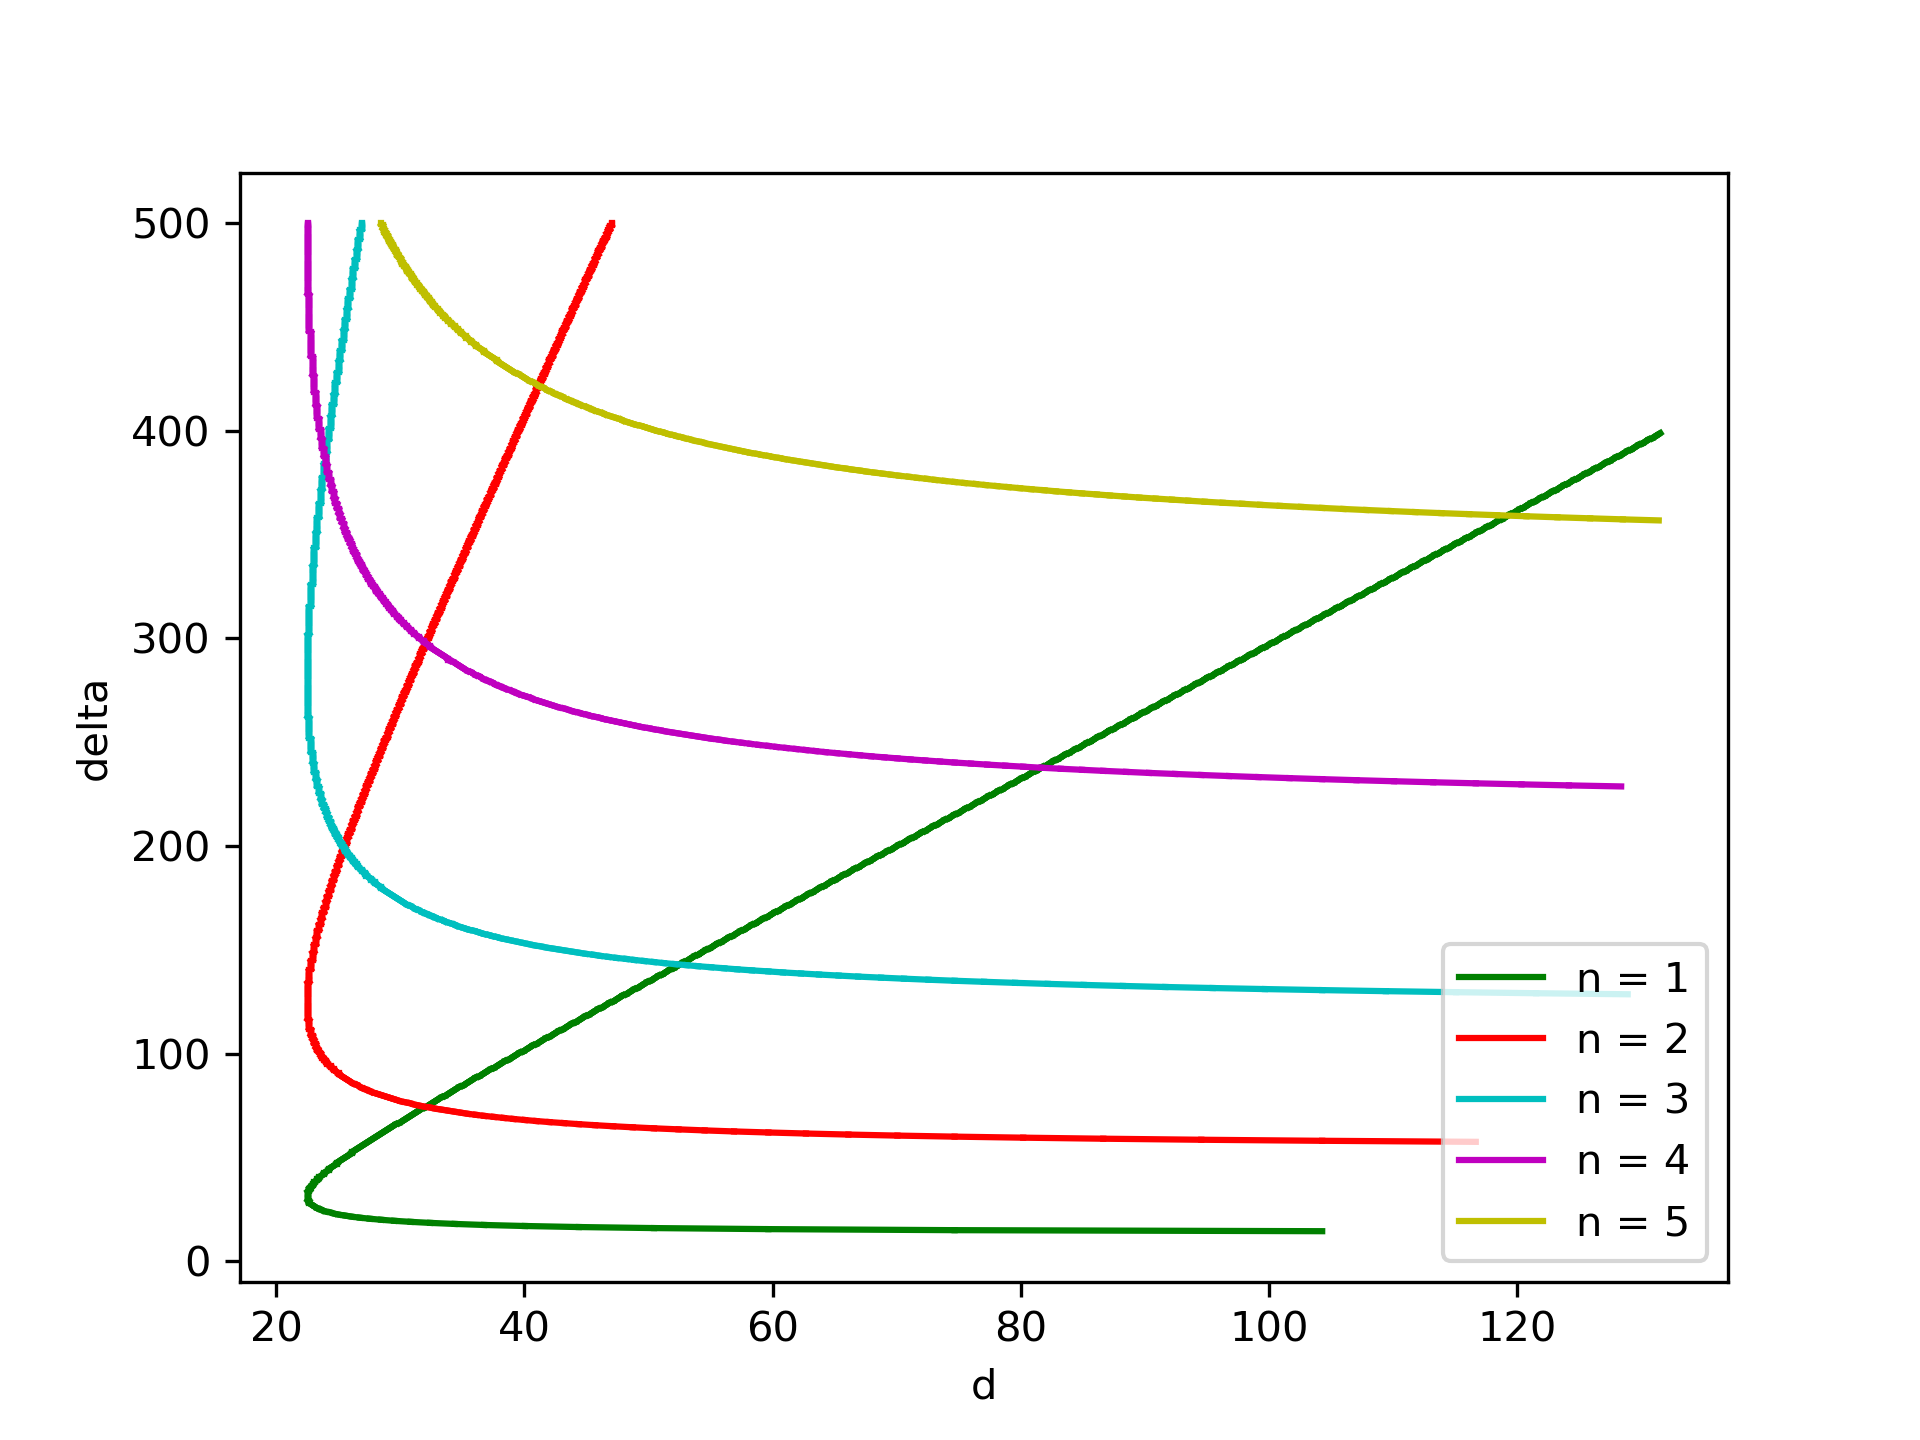
\includegraphics[scale=0.8]{diagrammes_turing_bis2.png}
\caption{Diagramme de Turing pour les modes 1 à 5}
\end{center}
\end{figure}

Lorsque les valeurs de $\delta$ et $d$ se trouvent à gauche de la courbe, alors la solution pour le mode en question est stable. Sinon elle est instable. On n'a pas tracé le mode $n=0$ car celui-ci est toujours stable (il correspond à la solution en l'absence de diffusion). Lorsque n est très grand, le terme de diffusion est prépondérant, et on a alors l'équation :
\begin{equation}
    \frac{ds_{n}}{dt} = -D(n\pi)^{2}s_{n}
\end{equation}
La solution d'équilibre de cette équation est elle-aussi toujours stable, ce qui est cohérent avec le graphique puisque les courbes "montent" lorsque n augmente. \\ \\
De plus, on observe que quelque soit le mode, les courbes atteignent toutes une valeur de d minimum que l'on va appeler $d_{critique}$.


\begin{figure}[h!]
\begin{center}
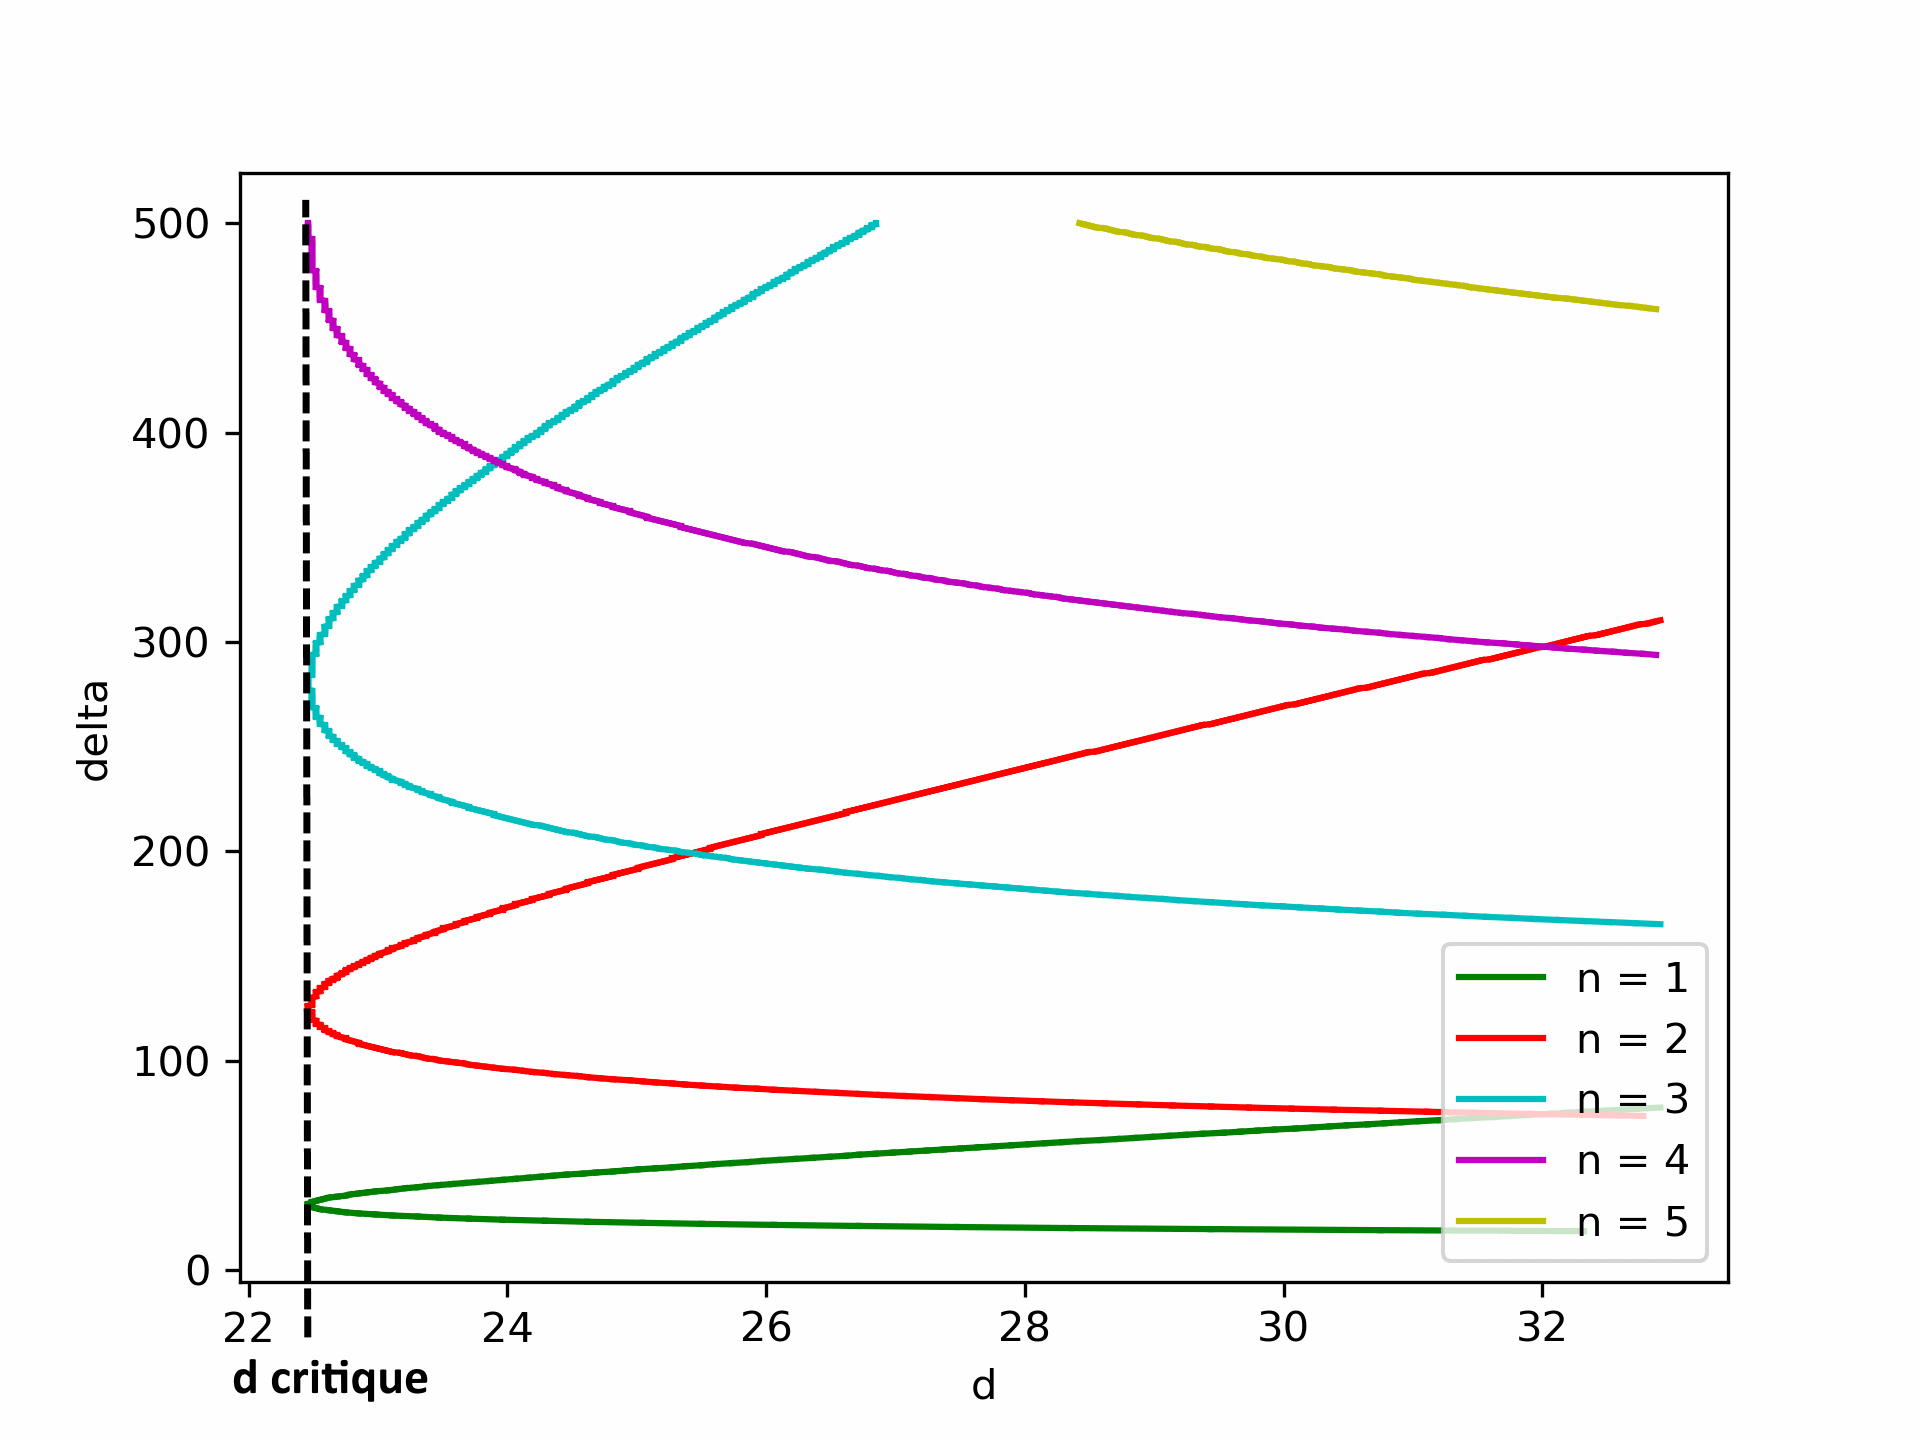
\includegraphics[scale=0.8]{diagrammes_turing_bis_avec_d_crit.png}
\caption{Diagramme de Turing pour les modes 1 à 5}
\end{center}
\end{figure}

Pour $d<d_{critique}$, alors tous les modes sont tous stables. La solution d'équilibre est donc totalement stable. \\ \\
Grâce à ce diagramme, étant données des valeurs de $\delta$ et $d$, on va pouvoir prédire quel mode va diverger, et quel mode sera stable.

\section{R\'esolution par la m\'ethode d'Euler implicite}
\textbf{Definition des variables et des param\`etres : }
On d\'efinit tout d'abord les diff\'erentes variables dont on a besoin pour d\'ecrire les \'equations du sch\'ema d'Euler implicite : \\
\begin{itemize}
	\item On fixe comme param\`etres $a = 0.2$ et $b = 1.3$ pour satisfaire les conditions $(a+b)^3>b-a$ et $b>a$.\\

	\item On appelle $N_x$ le nombre d'it\'erations sur la variable d'espace, avec $x$ variant entre 0 et 1, on a donc $dx = \frac{1}{N_x}$. On a pris ici $N_x = 30$.\\

	\item On garde la notation $c = \begin{pmatrix} u \\ v \end{pmatrix}$, qui sera de taille $2 N_x$.\\

	\item Le pas de temps doit \^etre assez petit, $dt = 10^{-3}$ suffit, en dessous, le sch\'ema diverge. On prend de plus une plage de temps suffisamment grande pour que les modes puissent appara\^itre, par exemple $N_t = 50 000$, voire plus si n\'ecessaire.\\

	\item Dans une variable $stock$ (tableau de taille $(2N_x,N_t)$)sont stock\'ees toutes les valeurs de $u$ et $v$.\\
\end{itemize}
\textbf{Initialisation autour de la solution d'\'equilibre : }\\
On se place autour de la solution d'\'equilibre, calcul\'ee comme \'etant $u_{eq} = a+b$ et $v_{eq} = \frac{b}{(a+b)^2}$, en ajoutant un nombre al\'eatoire compris entre $-10^{-4}$ et $10^{-4}$.
\begin{figure}[h]
\center{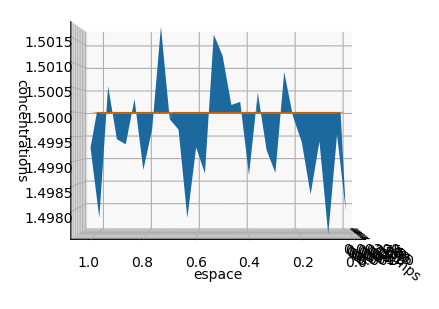
\includegraphics[scale = 0.8]{cond_init.png}}
\caption{Conditions initiales al\'eatoires autour de l'\'equilibre}
\label{fig cond init}
\end{figure}
\\

\textbf{Matrices du Laplacien et de Diffusion :}\\
Nous avons besoin de l'op\'erateur Laplacien discret dont la matrice, de taille  $(N_x, N_x)$, s'\'ecrit  : \\
\begin{displaymath}
Lp = \frac{1}{dx^2} \begin{pmatrix} 
-2     & 1     & 0      & \cdots & 1\\
 1     & -2    & \ddots & \ddots & \vdots\\
 0     &\ddots & \ddots & \ddots & 0\\
\vdots & \ddots& \ddots & \ddots & 1\\
1      &\cdots & 0      &    1   & -2
\end{pmatrix}
\end{displaymath}\\

Ce qui donne, \'ecrite par blocs ($1^{er}$ bloc appliqu\'e \`a $u$, le $2^{nd}$ \`a $v$):\\
\begin{displaymath}
A = \begin{pmatrix} 
Lp  & 0 \\
 0  & Lp
\end{pmatrix}
\end{displaymath}\\

Il nous faut \'egalement la matrice de diffusion, qui s'\'ecrit simplement par blocs, pour un coefficient de diffusion $d$ et en notant $I$ la matrice identit\'e de dimensions $(N_x, N_x)$ :\\
\begin{displaymath}
D = \begin{pmatrix} 
I  & 0 \\
 0  & dI
\end{pmatrix}
\end{displaymath}\\

Si on note $c^n = \begin{pmatrix} u^n \\ v^n \end{pmatrix}$ le vecteur $c$ \`a l'instant $t_n = n dt$, le sch\'ema d'Euler implicite s'\'ecrit :\\
\begin{equation}
c^{n+1} = c^n + dt (DA c^{n+1} + \delta f(c^{n+1}))
\end{equation}\\

On utilise ici un sch\'ema d'Euler simplifi\'e dans le sens o\`u on remplace $f(c^{n+1})$ par simplement $f(c^n)$. On obtient ainsi :\\
\begin{align}
c^{n+1} = c^n + dt (DA c^{n+1} + \delta f(c^n)) \nonumber\\
\nonumber \\
c^{n+1} = (I + dt DA)^{-1} (c^n + dt \delta f(c^n))
\end{align}\\

On it\`ere ainsi ce sch\'ema $N_t$ fois, et \`a chaque it\'eration, on stock le r\'esultat en remplissant la $n^{i\`eme}$ ligne de la matrice $stock$:\\
\begin{equation}
stock(n, 1:2 N_x) = c^n
\end{equation}\\
 
\textbf{R\'esultats : }\\

On se place \`a $d=30$ et $\delta= 120$. Sur le diagramme de Turing, on anticipe la stabilit\'e des deux premiers modes, et on s'attend \`a voir apparap\^itre le mode 2. C'est en effet ce que l'on observe : \\
\begin{figure}[h!]
\center{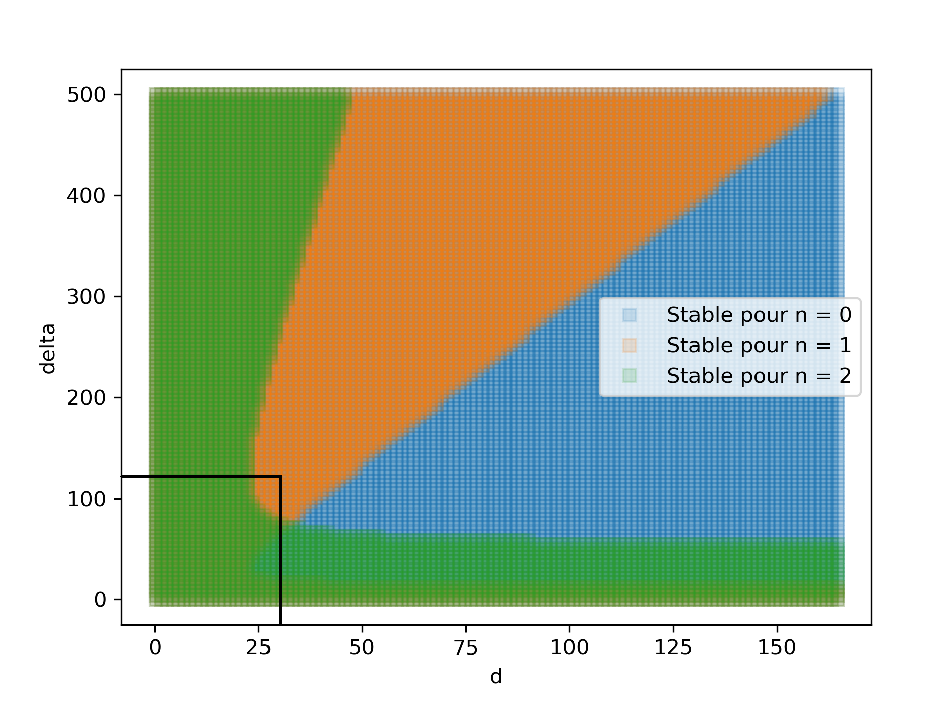
\includegraphics[scale = 0.25]{diagrammes_turing20-120.png}}
\caption{Diagramme de Turing : instabilit\'e du mode 2}
\label{fig turing1}
\end{figure}\\


\begin{figure}[h!]
\center{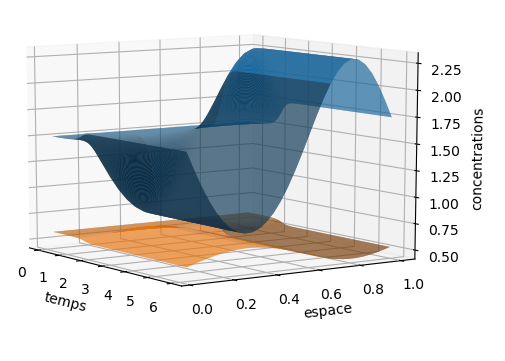
\includegraphics[scale = 0.7]{d30delta120.png}}
\caption{Concentrations u et v pour $d=30$ et $\delta = 120$}
\label{fig concentration1}
\end{figure}
On peut examiner d'autres cas, o\`u les modes instables se superposent  : \\

\begin{figure}[h!]
\center{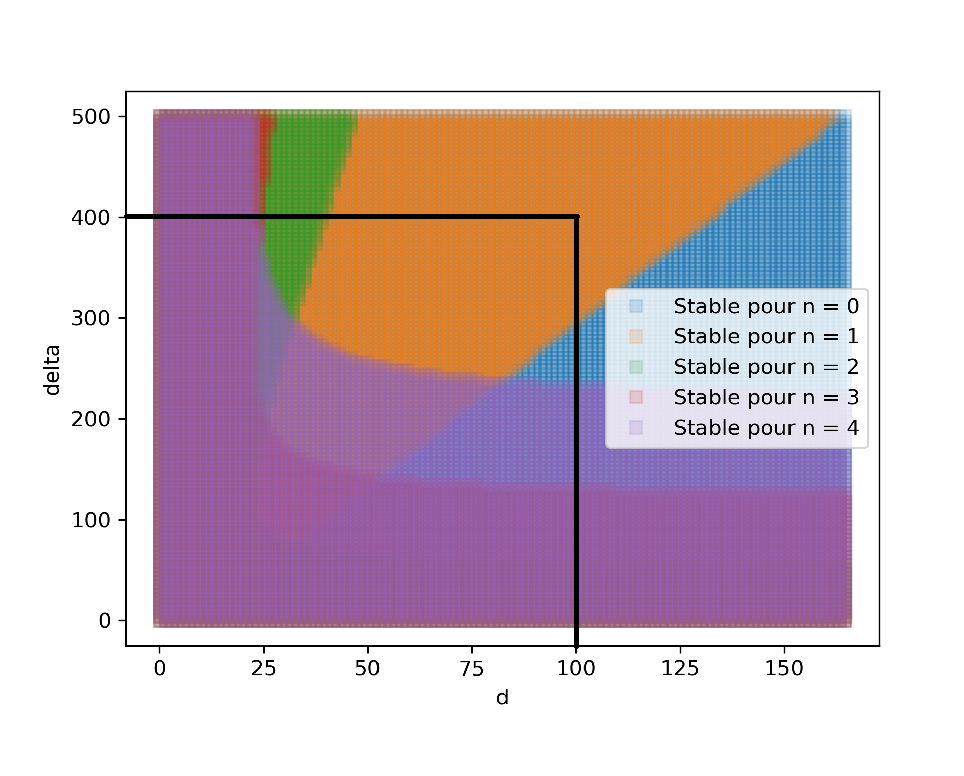
\includegraphics[scale = 0.25]{diagrammes_turing100-400.png}}
\caption{Diagramme de Turing : superposition de modes instables}
\label{fig turing2}
\end{figure}
\begin{figure}[h!]
\centering
\begin{subfigure}[h]{0.4\linewidth}
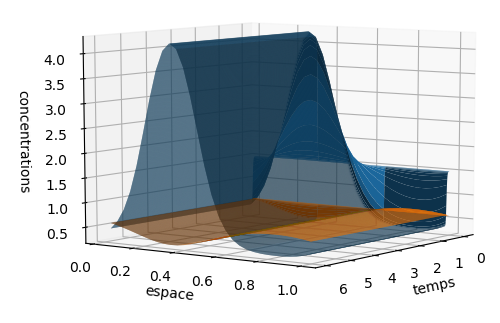
\includegraphics[width=\linewidth]{d100delta400.png}
  \end{subfigure}
  \begin{subfigure}[h]{0.4\linewidth}
    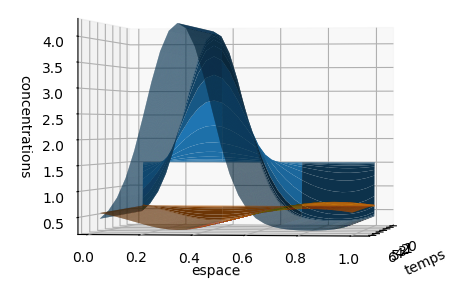
\includegraphics[width=\linewidth]{d100delta400_1.png}
  \end{subfigure}
  \caption{Concentrations pour $d=100$ et $\delta=400$}
  \label{fig concentration2}
\end{figure}


\begin{figure}[h!]
\center{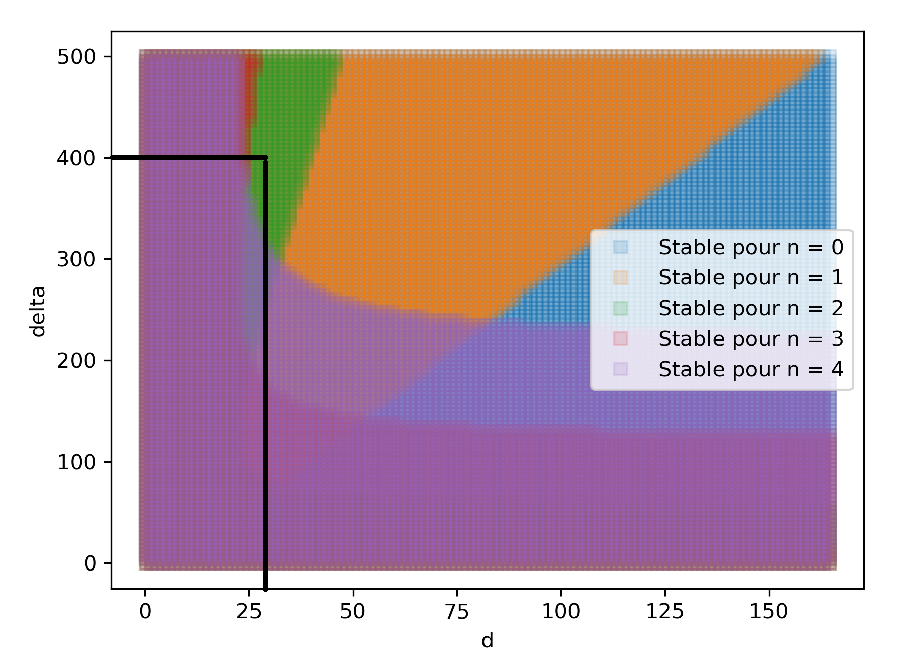
\includegraphics[scale = 0.25]{diagrammes_turing30-400.png}}
\caption{Diagramme de Turing : superposition de modes instables 2}
\label{fig turing3}
\end{figure}
\begin{figure}[h!]
  \centering
  \begin{subfigure}[h]{0.4\linewidth}
    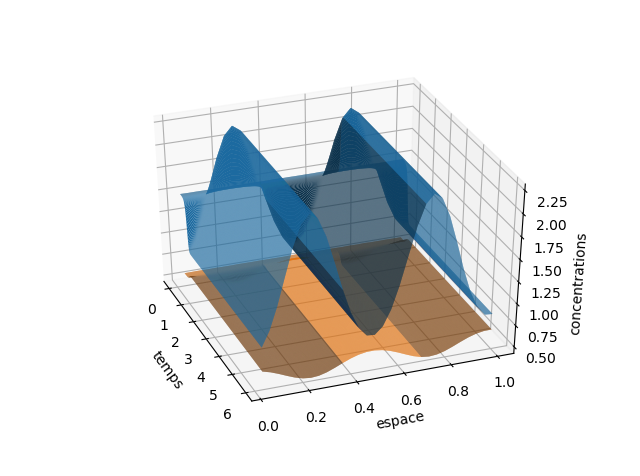
\includegraphics[width=\linewidth]{d30delta450.png}
  \end{subfigure}
  \begin{subfigure}[h]{0.4\linewidth}
    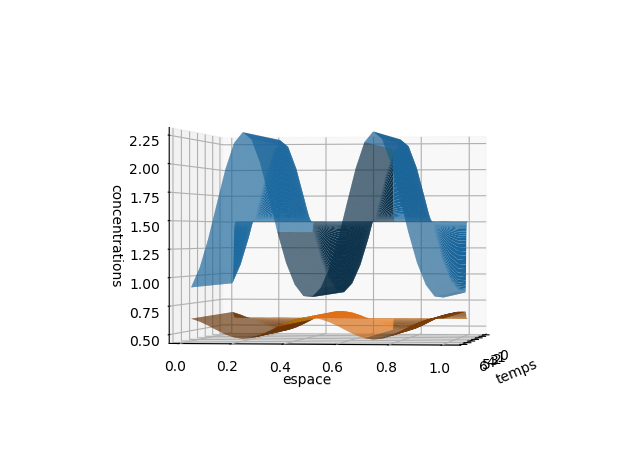
\includegraphics[width=\linewidth]{d30delta400_1.png}
  \end{subfigure}
  \caption{Concentrations pour $d=30$ et $\delta=400$ (mode 3 instable}
  \label{fig concentration3}
\end{figure}


\begin{figure}[h!]
\center{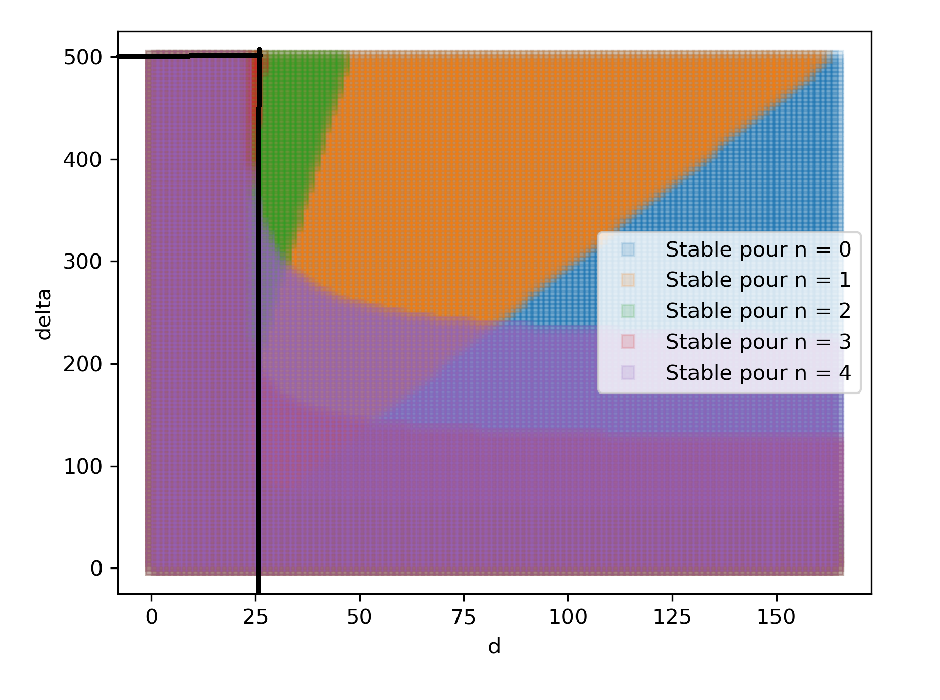
\includegraphics[scale = 0.25]{diagrammes_turing26-500.png}}
\caption{Diagramme de Turing : instabilit\'e du mode 4}
\label{fig turing1}
\end{figure}
\begin{figure}[h!]
\center{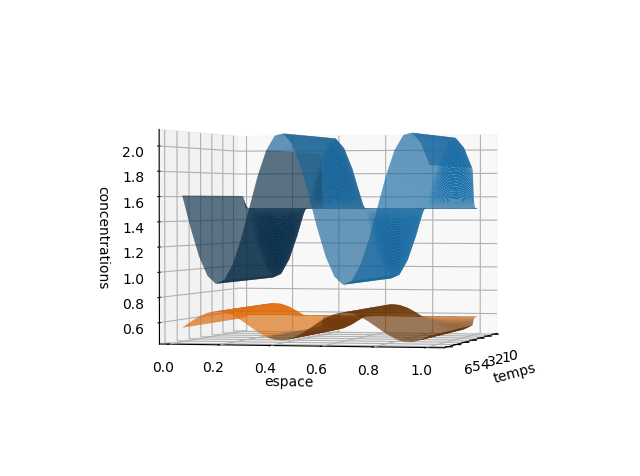
\includegraphics[scale = 0.7]{d26delta500.png}}
\caption{Concentrations u et v pour $d=26$ et $\delta = 500$ (mode 4 instable)}
\label{fig concentration4}
\end{figure}
Remarque : plus on est proche du $d_critique$, environ 23, plus les concentrations mettent du temps \`a converger vers une solution ind\'ependante du temps.\\
\begin{figure}[h!]
  \centering
  \begin{subfigure}[h]{0.4\linewidth}
    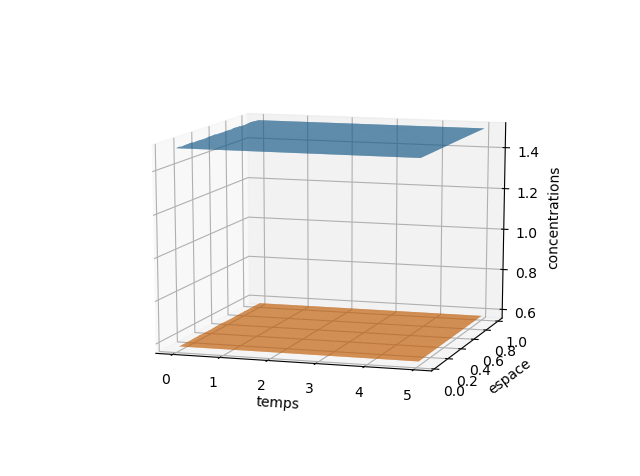
\includegraphics[width=\linewidth]{dcrit5.png}
  \end{subfigure}
  \begin{subfigure}[h]{0.4\linewidth}
    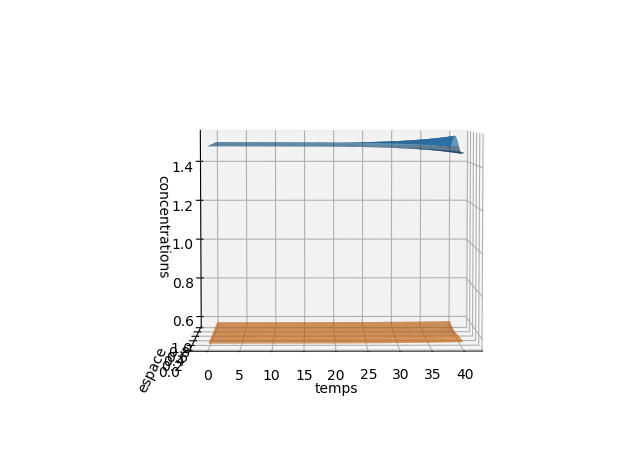
\includegraphics[width=\linewidth]{dcrit40.png}
  \end{subfigure}
	  \begin{subfigure}[h]{0.4\linewidth}
    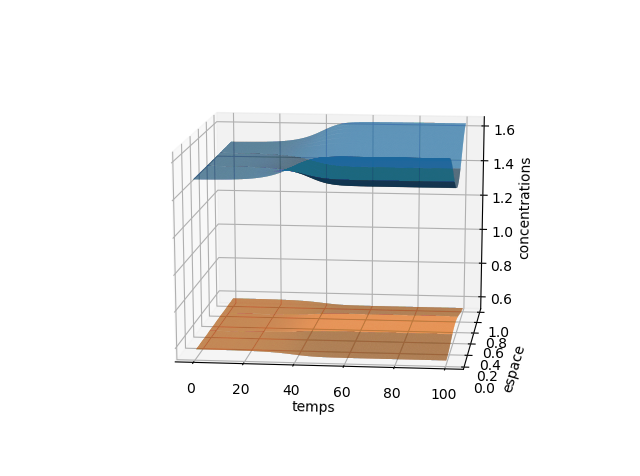
\includegraphics[width=\linewidth]{dcrit100.png}
  \end{subfigure}
  \caption{Concentrations pour $d=23.1$ et $\delta=150$ : convergence apr\`es 50 secondes de temps}
  \label{fig dcrit_tps}
\end{figure}


\subsection{Comparaison avec le diagramme de Turing théorique}
% ----------------- A RAJOUTER A LA FIN DE LA PARTIE DE DANA (EULER) ------------------
Maintenant que l'on a une méthode numérique pour résoudre l'équation, on va pouvoir comparer la stabilité de la solution d'équilibre pour des valeurs de $\delta$ et $d$ avec les résultats prédits par le diagramme de Turing théorique tracé à la section précédente. On sait que l'unique solution d'équilibre est $c_{eq} = (u_{eq},v_{eq}) = (a + b, \frac{b}{(a+b)^{2}})$. Une fois les paramètres fixés, on résout l'équation avec la méthode d'Euler sur une plage de temps suffisante pour que la solution se stabilise, puis on compare la solution au temps final avec la solution homogène en espace $c_{eq}$. Comme précédemment, on fait des boucles sur $\delta$ et $d$ et on trace un diagramme de stabilité. On trouve le résultat suivant (avec la zone stable en bleu), que l'on superpose avec le diagramme de Turing théorique :
\begin{figure}[h!]
\center{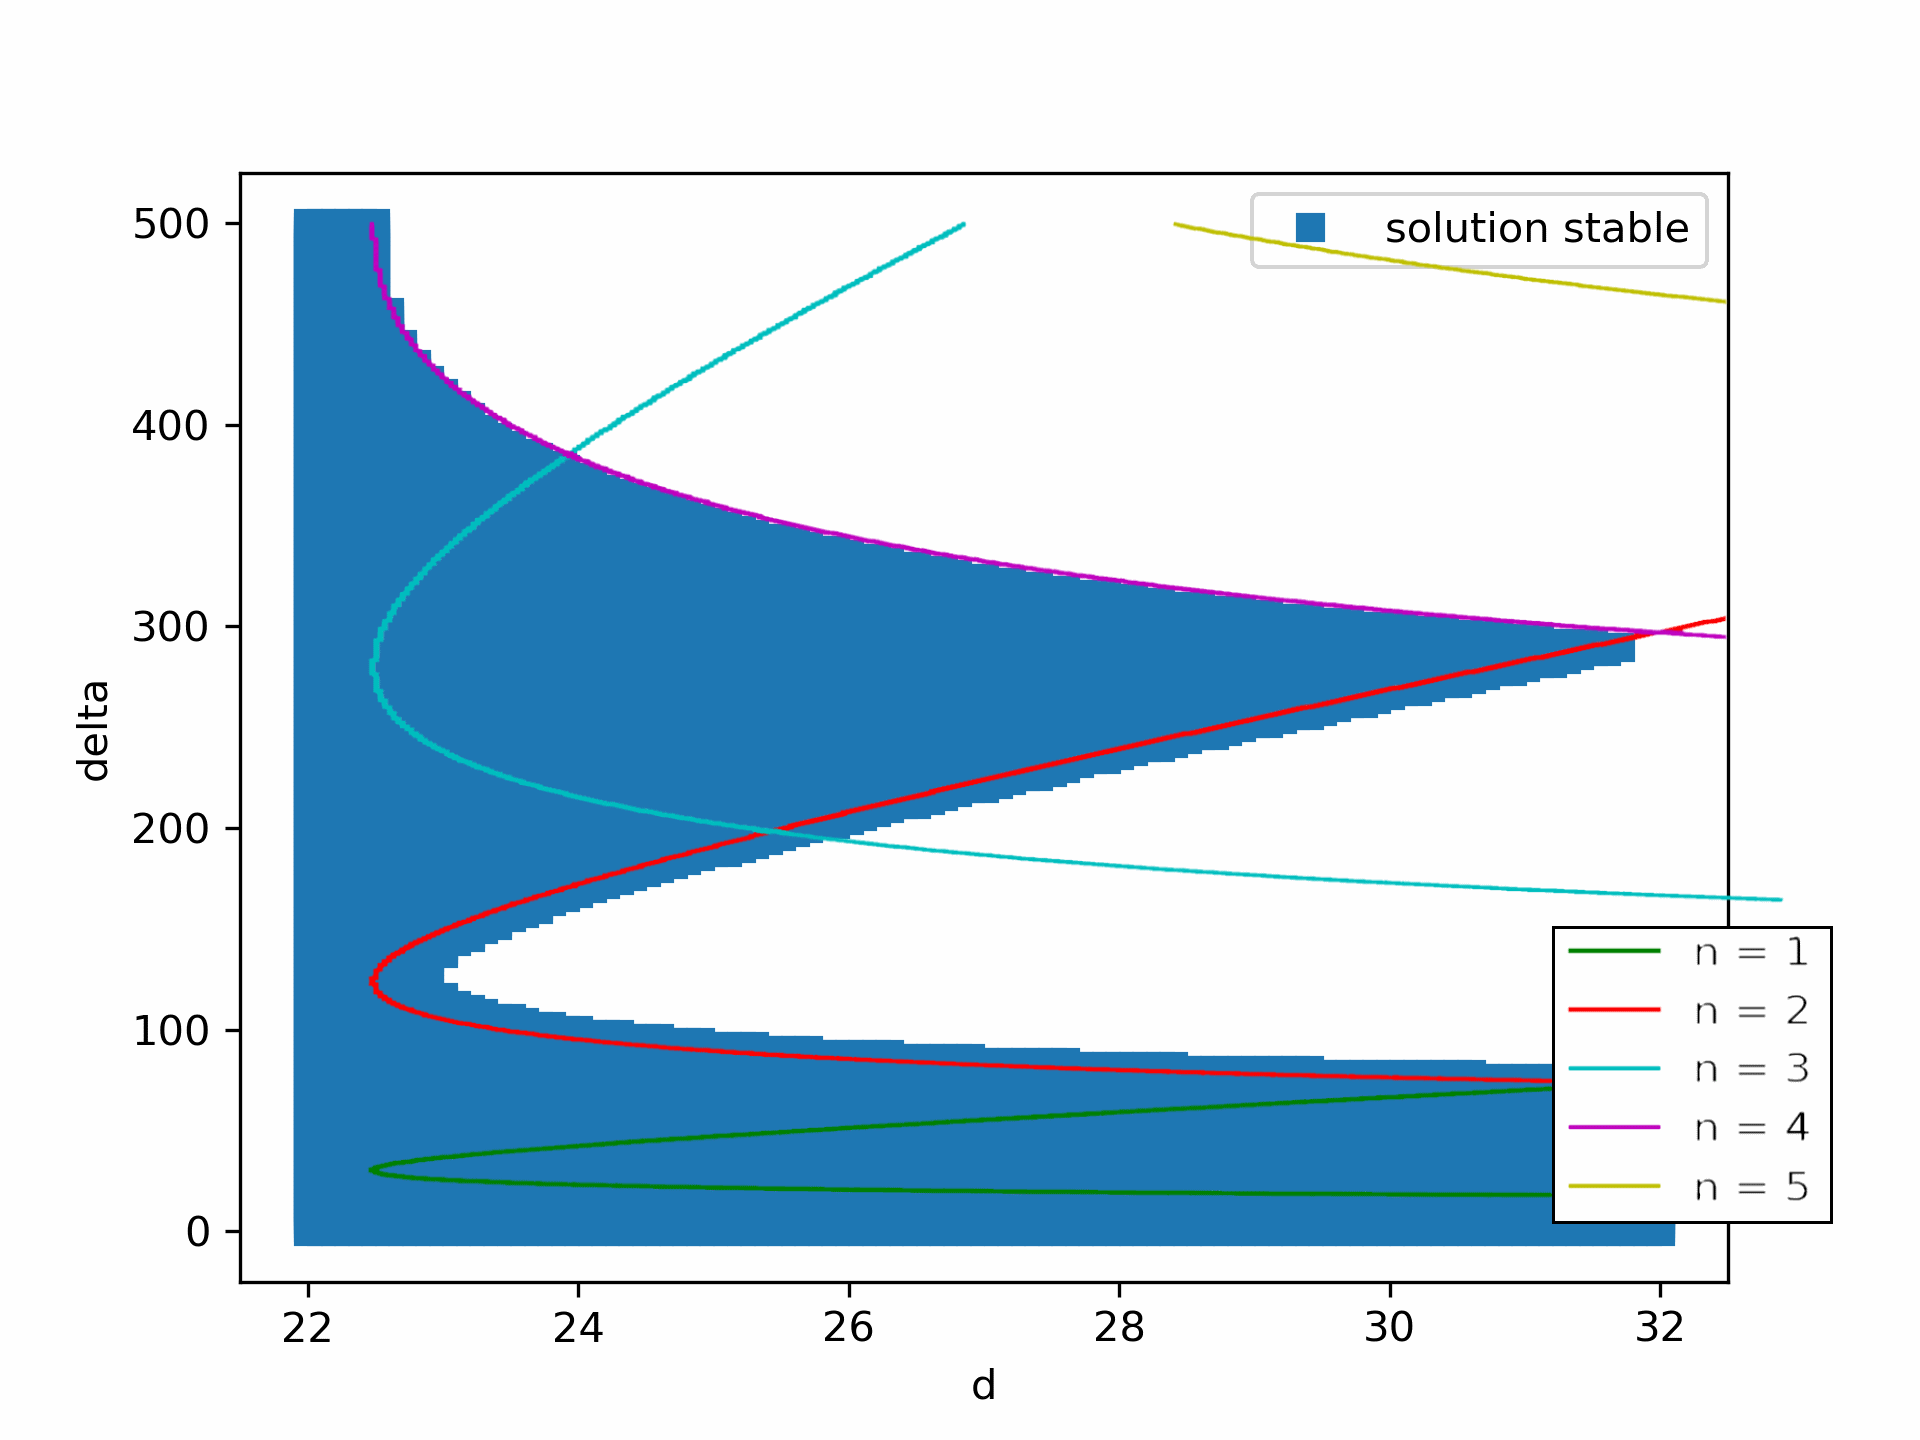
\includegraphics[scale = 0.8]{superposition_diagrammes_turing.png}}
\caption{Superposition des diagrammes de Turing théorique et expérimental}
\label{fig concentration1}
\end{figure}

On remarque que les deux diagrammes coïncident pour les modes 2 et 4, mais au niveau des modes 1 et 3, la résolution numérique donne une solution stable alors qu'elle ne devrait pas l'être. Cela peut être dû à des discrétisations trop grossières, ou un temps de résolution trop réduit, mais les temps de calcul déjà très importants ne permettent pas d'augmenter la précision du modèle.


\section{Amplitude des modes}
Dans cette partie nous nous intéressons à comment la forme de la solution évolue dans le temps lorsque nous plaçons le paramètre $d$ légèrement au dessus de $d_c$. Nous avons en effet remarqué au cours de nos simulations que pour certaines valeurs de $d$, la solution en $u$ s'apparentait à une sinusoïde de cette forme :
\begin{figure}[h!]
\center{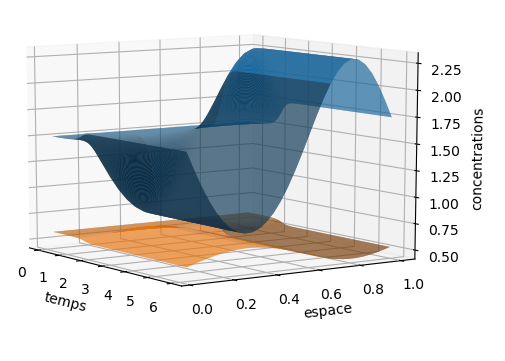
\includegraphics[scale = 0.7]{d30delta120.png}}
\caption{Concentrations u et v pour $d=30$ et $\delta = 120$}
\label{fig concentration1}
\end{figure}

À ce stade de notre étude nous souhaiterions donc retrouver ce résultat par une approche théorique. Ainsi nous considérons le paramètre $d$ choisi tel que :
\begin{equation}
d = d_c + \epsilon
\end{equation}
Pour $\epsilon \ll 1$, en pratique la pertubation $\epsilon$ sera de l'ordre de 0.05 au maximum. Le paramètre $\delta$ sera choisi plus arbitrairement car son influence sur la solution asymptotique est relativement limité, dans notre cas nous prendrons $\delta = 125$. Et de sorte que la solution asymptotique $c$ sera controlé par $\epsilon$ selon la forme d'une série : 
\begin{equation}
c(x) = \sum_{n=0}^{\infty} \epsilon^{\xi n} c_n (x)
\end{equation}
Où $\xi$ une constante réelle à caractériser dans la suite. Pour faire cela, utilisons l'équation : 
\begin{equation}
Dc''(x) + f(c)=0
\end{equation}
L'injection de la solution $c$ dans cette équation donne la nullité d'une nouvelle série similaire à $c$. Il suffit alors de regrouper les termes portant le même monôme en $\epsilon$, les deux premiers étant ceux d'ordre 0 et 1, imédiatement : \\

\begin{equation}
\left\{
    \begin{array}{ll}
        \begin{pmatrix}
        1 & 0\\
        0 & d_c
        \end{pmatrix} c_0'' + f(c_0) = 0
        \\
        \\
        \begin{pmatrix}
        1 & 0\\
        0 & d_c
        \end{pmatrix} c_1'' + df(c_0)c_1 = 0
    \end{array}
\right.
\end{equation}
\\

La première équation donne la solution d'équilibre, que l'on notera $\overline{c} $, pour $c_0$ comme on aurait pu s'y attendre d'après la simulation numérique. Pour la deuxième équation, il peut être intéressant d'écrire $c_1$ dans la base des fonctions cosinus. Une fois cela fait on tombe sur le même problème vu dans la section concernant les diagrammes de Turing, de plus pour la valeur choisi de $d$ on peut simplifier en remarquant qu'il existe un unique entier $j$ tel que le déterminant de la matrice $B_j$ soit nul. En effet, cela signifie que $c_1$ est forcément de la forme : 
\begin{equation}
c_1(x) = A cos(jx)e_j
\end{equation}
Où A est une constante réelle et $e_j$ le vecteur générateur du noyau de $B_j$.  En réalité on se doute que $j=2$, cela pourrait vraissemblablement être vérifié par un calcul numérique. À ce stade de la résolution, on peut raisonnablement penser que la constante $\xi$ est strictement positive, et que dans ce cas la solution $c$ s'approximerait assez bien par $\overline{c} + A \epsilon^{\xi} cos(jx)e_j$ ce qui confirmerait fortement nos résultats numérique. À présent un moyen de déterminer $\xi$ est d'utiliser les ordres suivant sachant les conditions trouvées sur $c_0$ et $c_1$. \\

À cause du terme $d_c + \epsilon$ dans la matrice de diffusion, un terme porté par $\epsilon^{\xi +1}$ apparait : 
\begin{equation}
\epsilon^{\xi +1} v_1 ''   \begin{pmatrix}
        1 \\
        0 
        \end{pmatrix} 
\end{equation}
À supposer que $\xi +1$ ne s'écrive pas sous la forme $n\xi$, alors le terme ci-dessus est le seul d'ordre $\xi +1$ et donc est nul. Or cela est contradictoire avec la forme trouvée de $c_1$. Nécessairement, il existe $n$ entier supérieur ou égal à 2 tel que $\xi+1=n\xi$. En ne rentrant pas plus dans le détail, il s'agit ici d'exploiter l'alternative de Fredholm pour montrer que la seule possibilité est que le terme d'ordre $\xi+1$ doit se méler à celui en $3\xi$. Cela donne $\xi=\frac{1}{2}$ et donc : 
\begin{equation}
c(x) = \sum_{n=0}^{\infty} (\sqrt{\epsilon})^n c_n (x)
\end{equation}
Par ailleurs, l'alternative de Fredholm montre que la constante A vaut soit $0$, soit $\pm A_0$ où $A_0$ est une constante caractéristique de la fonction $f$. Enfin, nous avons :
\begin{equation}
c(x)\simeq\overline{c} \pm A_0 \sqrt{\epsilon} cos(jx)e_j
\end{equation}
\subsection{Confirmation par simulation}
On peut aller plus loin en tentant numériquement de retrouver cette dépendance en $\sqrt{\epsilon}$. Voici des résultats de plusieurs simulations : 
\begin{figure}[h!]
\centering
% Inclusion d'une image: ce qui est entre crochets est un argument "optionnel", alors que l'argument obligatoire est entre accolades
\includegraphics{graphique5}
\caption{\'Evolution de l'amplitude en fonction de $\epsilon$ et $\sqrt{\epsilon}$
         \label{fig:exemple}}
\end{figure}
En théorie la deuxième ligne de graphiques est censée représenter des graphes de fonctions linéaires or pour $\epsilon$ proche de 0 ce n'est pas ce qu'on observe. Les premiers graphes auraient du présenter une courbe plus redressée pour des valeurs proches de 0. Cependant la tendance asymptotique semble mieu correspondre les résultats théoriques, si on exploite cette partie de la courbe en $\sqrt{\epsilon}$, on trouve une pente d'environ $0,5$.

\section{Conclusion} 
Euuuh...
\end{document}
